\section{Evaluation}
\para{Implementation.}
The experiment setting is shown in Figure \ref*{fig:expset}. We implemented the system using a smart phone and a headgear holder. The smart phone works as a RGB camera for capturing real-time RGB images. Since the camera is fixed on the headgear holder, we can assume that the orientation of the camera lens is basically the same as the orientation of the user's face.


\begin{figure}[t]
	\begin{center}
		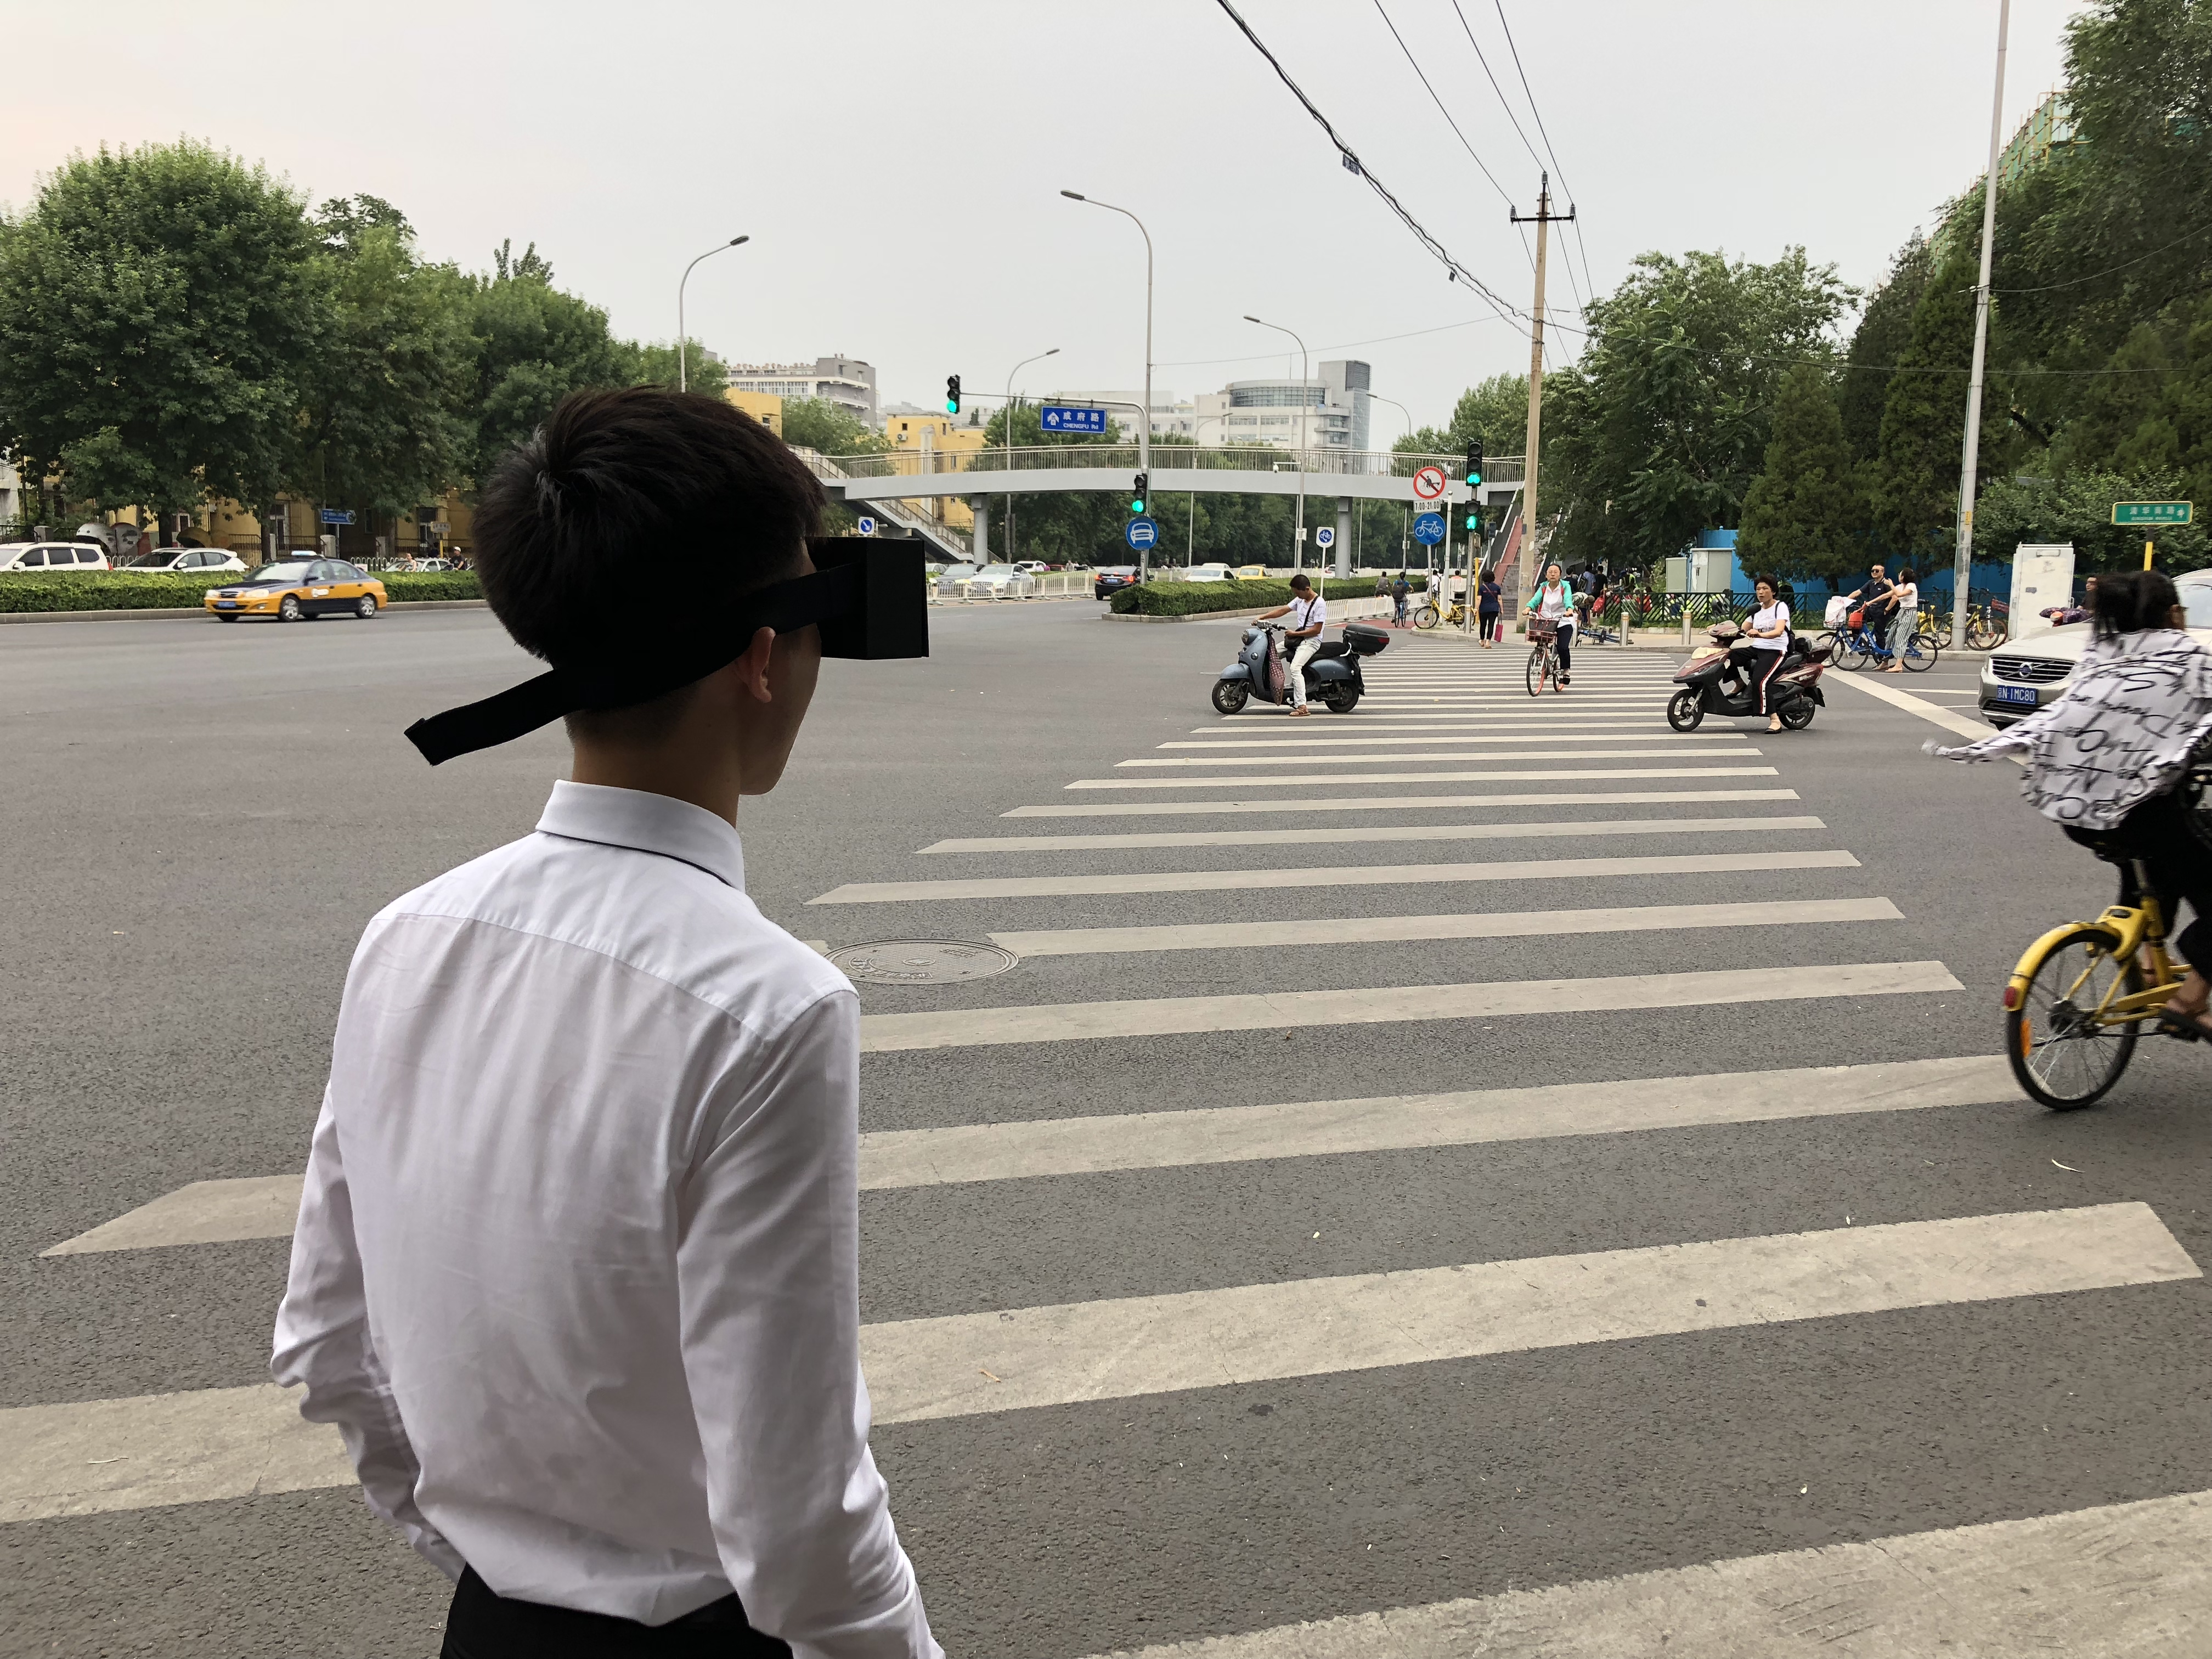
\includegraphics[width=1.\linewidth]{figure/experiment_setting.jpg}
	\end{center}
	\caption{Experiment setting: the user is wearing a RGB camera.}
	\label{fig:expset}
\end{figure}


\para{Results.}
To evaluate the performance of the system, we select a series of representative scenarios from urban road scenes. The properties of the benchmark videos are shown in Table \ref{Table:Benchmarks}. Precision and recall are used as key indicators of the results. The results are shown in Table.  


\begin{table}[!t]
	\centering
	\caption{\footnotesize Properties of the Benchmark Videos}
	\label{Table:Benchmarks}
	%\begin{tabular}{c|c|c}
	 \begin{tabular}{p{1cm}p{4.5cm}p{2cm}}	
		\hline
		Scenario &    Description      &  Total Frames         \\ \hline \hline
		1        &    The red light turns green or the green light turns red. The lights are visible throughout the journey. There is only one pedestrian light in the scene.      &      189    \\ \hline  %video1
		2        & There are multiple traffic lights in the scene. The non-pedestrian lights change their colos (e.g. red to green or green to red). &      162       \\ \hline  %video4
	    3     	 & The zebra crossing is occluded in the distance and the pedestrian light exists in the scene.     &      133       \\ \hline   %video7
		4        & Zebra crossing is in the shade.  &     300      \\ \hline   %video9
		5        & Obstacle avoidance test: pedestrians walk nearby in the same direction. &    258        \\ \hline %video10
		6        & Obstacle avoidance test: pedestrians walk nearby in the opposite direction.   &       271      \\ \hline  %video11
		7        & Obstacle avoidance test: The vehicle is moving laterally in front.   &      340       \\ \hline  %video12
		8        & Pedestrians walk across the road and the pedestrian light stays green for the whole journey.   &       585      \\ \hline  %video15
		9        & Pedestrians walk across the road and the pedestrian light doesn't stay green for the whole journey.   &        158     \\ \hline  %video16
	\end{tabular}
\end{table}









\begin{table}[!t]
	\centering
	\caption{\footnotesize Evaluation Results}
	\label{Table:Results}
	\renewcommand{\multirowsetup}{\centering}
	\begin{tabular}{c|c|c|c|c}
	%\begin{tabular}{p{1cm}p{4.5cm}p{2cm}}	
		\hline
		\multirow{2}[0]{*}{Scenario}  &   \multicolumn{2}{c|}{Detection}    &    \multicolumn{2}{c}{Detection+Tracking}      \\ \cline{2-5}
		 &    Precision      &  Recall   &  Precision & Recall     \\ \hline \hline
		1        &  &    & &            \\ \hline  %video1
		2        &  &    & &            \\ \hline  %video4
		3     	 &  &    & &           \\ \hline  %video7
		4        &  &    & &           \\ \hline  %video9
		5        &  &    & &           \\ \hline  %video10
		6        &  &    & &           \\ \hline  %video11
		7        &  &    & &          \\ \hline  %video12
		8        &  &    & &          \\ \hline  %video15
		9        &  &    & &          \\ \hline  %video16
	\end{tabular}
\end{table}